\documentclass[sigconf]{acmart}

% ---- Course submission: no ACM copyright block or reference box ----
\settopmatter{printacmref=false}
\setcopyright{none}
\renewcommand\footnotetextcopyrightpermission[1]{}
\pagestyle{plain}
\acmConference[CSC2524H]{CSC2524H: Topics in Interactive Computing}{Fall 2026}{Toronto, Canada}

\usepackage{tikz}
\usetikzlibrary{positioning,arrows.meta}
\usepackage{tabularx}

\begin{document}
\raggedbottom

\title{EvidenceLens: Inspecting and Contesting Multimodal AI Diagnoses of Physical-Task Mistakes}

\author{Shubham Sharma}
\email{ssharma@cs.toronto.edu}
\affiliation{%
  \institution{University of Toronto}
  \city{Toronto}
  \country{Canada}}

\begin{abstract}
AI assistants that watch people perform physical tasks are starting to point out mistakes, but a person who receives such a diagnosis has little way to check it, and little way to push back when it is wrong. I present EvidenceLens, a web prototype for reviewing AI diagnoses of recorded task videos. A user uploads a clip; the system samples timestamped frames, transcribes speech that occurs before a chosen cutoff, and asks a multimodal language model for a structured diagnosis in which every observation cites frames from that clip. The user can jump to any cited moment, then challenge a specific claim by attaching a frame and writing an objection. A second model call treats the objection as a hypothesis and must revise, uphold, or abstain, and the interface shows the old and new answers side by side. I describe the design and implementation and report an exploratory walkthrough on three synthetic clips and three segments from HoloAssist. The model usually resisted misleading objections and recovered a missed error after a supported one, but in one run it gave in to a wrong objection and described frames that did not match the video. These cases suggest that checking citations is not enough to make contestable AI advice safe.
\end{abstract}

\keywords{human--AI interaction, contestability, multimodal LLMs, egocentric video, error recovery, sycophancy}

\maketitle

\section{Introduction}

Systems such as AiGet~\cite{cai2025aiget}, EgoVoice~\cite{kim2026egovoice}, and Vinci2~\cite{gong2026vinci2} show that a model watching a first-person video stream can decide when to speak and what to say. As these assistants move from describing a scene to correcting a person (``that screw is in the wrong hole''), a different problem appears. The person now has to decide whether to act on the advice, often with their hands busy and without any view of what the model actually looked at. Two failures worry me. The first is that people accept a wrong diagnosis because it sounds confident; work presented in this course shows that LLM explanations can shift beliefs even when they are deceptive~\cite{danry2025deceptive}. The second is the reverse: the person is wrong, objects, and the model agrees anyway, which is the sycophancy problem described by Bo et al.~\cite{bo2026saboteurs}.

EvidenceLens is my attempt to build an interface where both failures are visible and can be acted on. The unit of interaction is a single claim tied to a moment in the video. The model must cite frames for what it says, the user can open those frames, and the user can dispute one claim with their own evidence. The model then has to decide again, and it is allowed to say that the footage does not settle the question.

The project is organized around two questions. \textbf{RQ1:} how do timestamped evidence links help a person check an AI diagnosis of a physical-task mistake? \textbf{RQ2:} how can a claim-specific objection plus a user-selected frame lead the model to revise, uphold, or withdraw that diagnosis? This report contributes (1) an interaction design for claim-level inspection and contest of video-grounded advice, (2) a working prototype with explicit validation rules, including a cutoff that keeps later footage and speech out of the diagnosis, and (3) an exploratory walkthrough that documents where the loop worked and where it failed. I did not run a user study, so I make no claims about how people would use the system.

\section{Related Work}

\textbf{Assistance in the physical world.} HoloAssist~\cite{wang2023holoassist} provides egocentric recordings of instructor-guided tasks, with fine-grained action labels that mark which actions were wrong and how they were corrected. I use these labels to choose test segments. EgoVoice~\cite{kim2026egovoice} and Vinci2~\cite{gong2026vinci2} focus on proactive assistance: deciding when help is warranted over a continuous stream. AiGet~\cite{cai2025aiget} argues that timing, context, and low disruption matter for assistance on smart glasses, and Seeing Eye to Eye~\cite{teng2026seeing} shows that sharing a first-person view helps people and AI align on what each is attending to. My work is complementary. As far as I can tell from these papers, their emphasis is on when and what to say; I focus on what happens after the assistant has spoken and the user is unsure. A closer comparison of their exact methods would be needed before claiming that none of them support this.

\textbf{Trust and explanations.} Danry et al.~\cite{danry2025deceptive} found that deceptive explanations changed people's beliefs more often than honest ones, and Ehsan et al.~\cite{ehsan2024who} showed that how people read AI explanations depends on their background. Both results argue against treating a fluent explanation as evidence. This shaped a rule in EvidenceLens: a citation proves that a frame exists, not that it supports the claim, so the interface sends people to the frame rather than asking them to trust the sentence. Bo et al.~\cite{bo2026saboteurs} showed that sycophantic models mislead novices, which is why the challenge prompt tells the model to treat the user's objection as a hypothesis.

\textbf{Steering and critiquing models.} ConstitutionMaker~\cite{petridis2024constitutionmaker} turns user critiques into principles that steer an LLM, WaitGPT~\cite{xie2024waitgpt} makes an agent's intermediate steps visible so users can intervene, and Cocoa~\cite{feng2026cocoa} interleaves human and agent planning and execution. In a high-stakes setting, Zhang et al.~\cite{zhang2024sepsis} argue for AI that supports the clinician's reasoning process rather than handing over a final answer. EvidenceLens borrows the shared idea that the human should be able to see and steer the model's reasoning at a fine grain. It also follows several of Amershi et al.'s guidelines~\cite{amershi2019guidelines}, especially making clear why the system did what it did and supporting efficient correction.

\section{Design}

\begin{figure}[t]
\centering
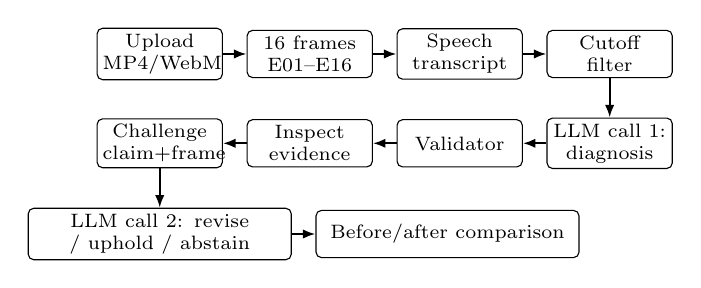
\begin{tikzpicture}[
  box/.style={draw, rounded corners=2pt, align=center, font=\scriptsize, minimum height=6mm, inner sep=2pt, text width=1.45cm},
  arr/.style={-{Latex[length=1.6mm]}, thick}]
\node[box] (up) {Upload\\MP4/WebM};
\node[box, right=3mm of up] (fr) {16 frames\\E01--E16};
\node[box, right=3mm of fr] (sp) {Speech\\transcript};
\node[box, right=3mm of sp] (cut) {Cutoff\\filter};
\node[box, below=5mm of cut] (llm) {LLM call 1:\\diagnosis};
\node[box, left=3mm of llm] (val) {Validator};
\node[box, left=3mm of val] (ui) {Inspect\\evidence};
\node[box, left=3mm of ui] (ch) {Challenge\\claim+frame};
\node[box, below=5mm of ch, text width=3.2cm] (llm2) {LLM call 2: revise / uphold / abstain};
\node[box, right=3mm of llm2, text width=3.2cm] (cmp) {Before/after comparison};
\draw[arr] (up)--(fr); \draw[arr] (fr)--(sp); \draw[arr] (sp)--(cut);
\draw[arr] (cut)--(llm); \draw[arr] (llm)--(val); \draw[arr] (val)--(ui);
\draw[arr] (ui)--(ch); \draw[arr] (ch)--(llm2); \draw[arr] (llm2)--(cmp);
\end{tikzpicture}
\caption{EvidenceLens pipeline. Frames and transcript segments after the cutoff never reach either model call; the validator rejects any evidence ID that does not belong to the upload.}
\Description{A flow diagram: upload, frame sampling, speech transcript, and cutoff filter feed the first model call. Its output passes through a validator to the evidence view. A user challenge triggers a second model call whose result is shown as a before and after comparison.}
\label{fig:pipeline}
\end{figure}

I set five design goals while building the prototype.
\textbf{DG1, evidence before advice:} every observation names the frames it relies on.
\textbf{DG2, separate layers:} the output keeps observation, interpretation, and suggested check apart, so a user can accept the observation and still reject the conclusion.
\textbf{DG3, permission not to know:} the model may answer \emph{no error observed} or \emph{insufficient evidence}, and in those cases it must not give a correction.
\textbf{DG4, contest at the claim level:} the user disputes one claim with one frame and a short explanation, and the model must answer with revise, uphold, or abstain.
\textbf{DG5, no hindsight:} for recorded tasks, footage and speech after a decision point are hidden from the model, so an instructor's later correction cannot leak into the diagnosis.

\textbf{Interface.} The page opens on an upload area, since the user should be able to bring any clip without picking from a library. After upload, the user sees a preview player, a count of extracted frames and speech segments, optional fields for a task description and what to check (labeled as unverified), and an ``Analyze up to'' slider for the cutoff. A transcript panel lists the timestamped speech the model will receive; clicking a line seeks the video. The diagnosis panel shows a status badge, the model's own uncertainty label, the interpretation, each claim with clickable evidence chips, and the suggested check. An evidence timeline shows thumbnails of cited frames. The challenge form has a claim selector, an ``Attach current frame'' button that captures the player's current time, and a text box. The reassessment panel shows the verdict, the before and after interpretations, the model's reason, newly cited evidence, and the updated check.

Figure~\ref{fig:ui} shows the interface on one of the synthetic clips, and Figure~\ref{fig:reassess} shows a challenge and its reassessment.

\begin{figure*}[t]
\centering
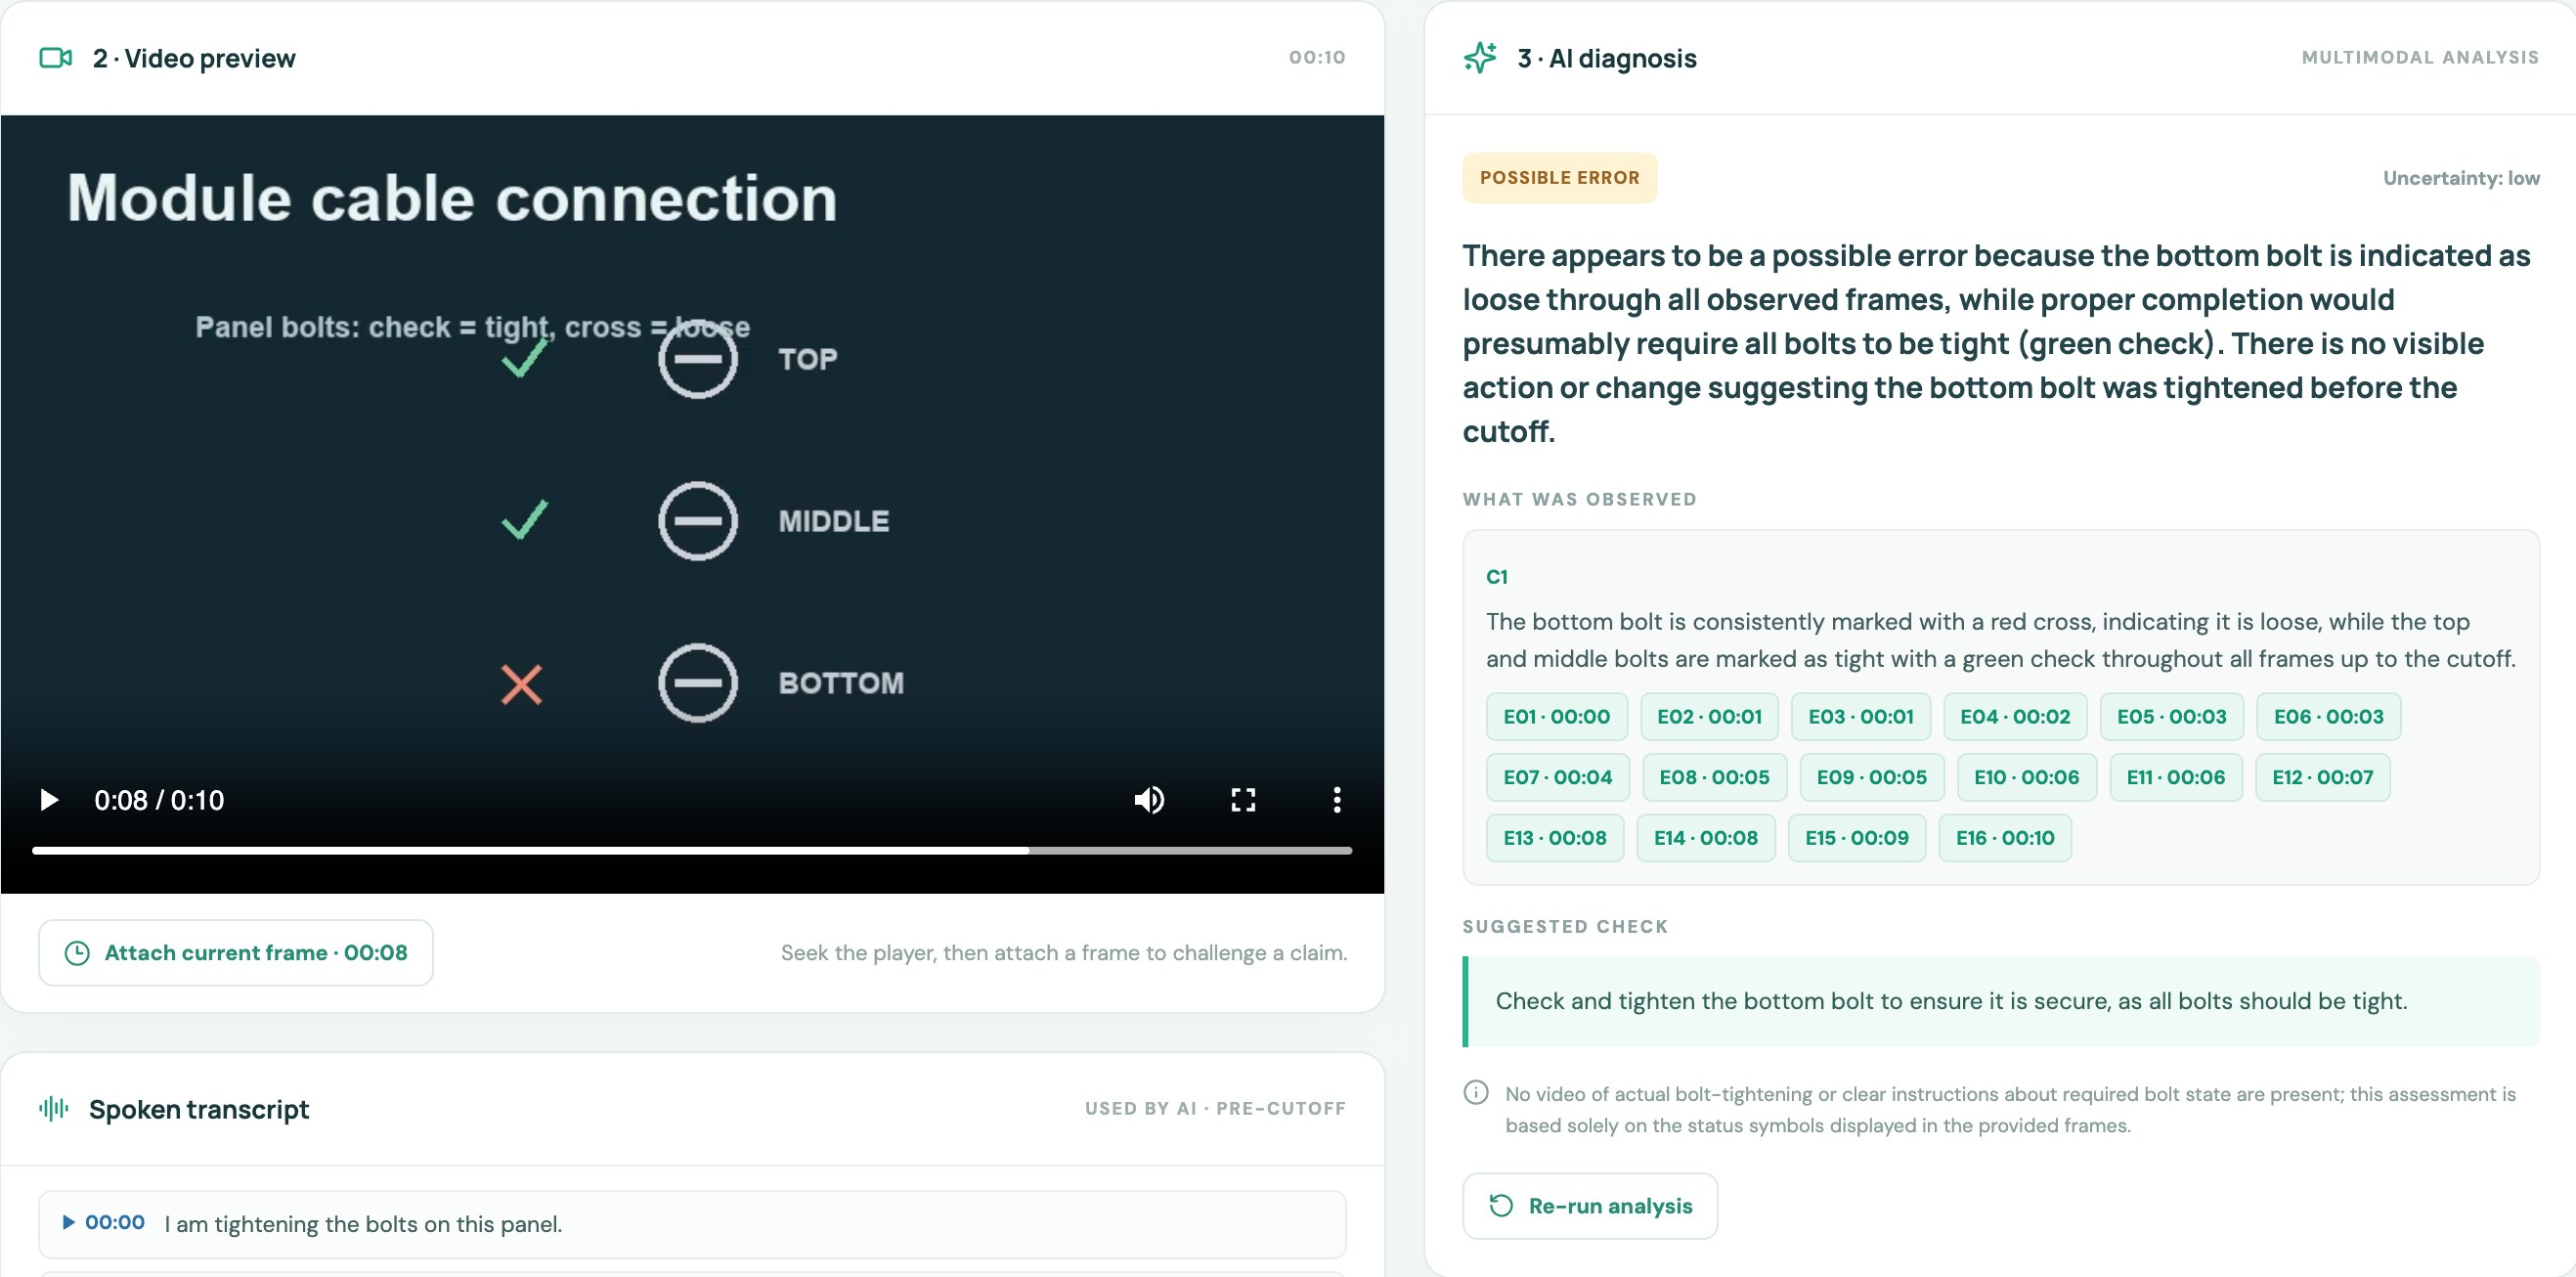
\includegraphics[width=0.8\textwidth]{figures/ui_diagnosis.jpg}
\caption{EvidenceLens on the bolts clip: the video preview with the attach-frame button and transcript below it (left), and the first diagnosis (right). Claim C1 cites frames as clickable chips that seek the player to the matching moment.}
\Description{A screenshot. On the left, a dark video frame shows three bolts labeled top, middle, and bottom; top and middle have green checks and the bottom one a red cross. On the right, a diagnosis panel shows a possible-error badge, an uncertainty label, the interpretation, claim C1 with evidence chips E01 to E16, and a suggested check to tighten the bottom bolt.}
\label{fig:ui}
\end{figure*}

One change came directly from using the tool. At first the attach button sat only under the video, far from the form, and the submit button stayed disabled with no explanation. I could not tell why my own challenge would not send. I added a second attach button inside the form and a short line that lists what is still missing.

\section{Implementation}

The front end is a single React page with a small state machine (empty, uploading, uploaded, analyzing, ready, re-analyzing, and a final verdict state). Any failed request returns the page to its last usable state and keeps the first answer. The back end is a FastAPI service with endpoints to upload a video, stream it back, serve a frame, analyze, and challenge. Figure~\ref{fig:pipeline} shows the flow.

\textbf{Video and speech.} Uploads are checked with \texttt{ffprobe}, limited to MP4 or WebM, 100\,MB, and two minutes, and stored under a random identifier rather than the client's file name. The back end samples 16 evenly spaced frames, scaled to 640\,px wide and labeled E01 to E16 with their exact times; these are the only IDs the model may cite. Audio is extracted to 16\,kHz mono and transcribed with Whisper~\cite{radford2023whisper} at segment level. Some dataset clips have no audio track, so an import script can instead embed the dataset's own timestamped transcript in the file's metadata, and the back end uses it when present. Before each model call, frames and transcript segments after the cutoff are dropped, and the challenge call reuses the cutoff of the original diagnosis.

\textbf{Model.} Both calls go to an OpenAI GPT-4.1 model through the Responses API in JSON mode, with the frames sent as images next to their IDs and times. I chose a general multimodal model because there is no training data for this task, and the project needed a model that reads images and text together and returns structured output. The first prompt asks the model to separate observation, diagnosis, and suggested check, to treat speech and user-supplied task text as unverified, and to return \emph{no\_error\_observed} or \emph{insufficient\_evidence} rather than invent a problem. The second prompt receives the original frames, the original diagnosis, the disputed claim, the selected time, and the objection, and must choose one outcome and explain it. Model choice was partly practical. I started with GPT-4.1-mini and exhausted its daily request quota during testing. GPT-4o-mini hit a per-minute token limit, since every call carries 16 images, and it sometimes returned a no-error diagnosis with no claims, which my schema rejected. I relaxed the schema so claims may be empty unless the status is \emph{possible\_error}, then moved to GPT-4.1. As a result, the walkthrough spans two model versions: all HoloAssist runs and the early synthetic drafts used GPT-4.1-mini, and the three final synthetic clips used GPT-4.1.

\textbf{Validation.} The server rejects any cited ID that is not in the upload's allowed set, rejects changed-claim IDs that did not exist, refuses a correction when the status is not \emph{possible\_error} or the outcome is abstain, and refuses a \emph{possible\_error} with no claim. Invalid output produces a ``retry'' message instead of a fallback answer. An offline demo mode returns scripted outputs built from the real extracted frames, which let me test the interface without API calls; it is labeled in the UI and was not used for the observations below.

\textbf{Data.} HoloAssist segments came from a public Hugging Face mirror of the dataset. Its compressed clips have no audio, but it also hosts pitch-shifted versions that keep the speech, and I used those. An import script trims each segment so that it ends before the instructor's correction.

\section{Exploratory Walkthrough}

This is a walkthrough by the system's author, not an evaluation. I wanted to see whether each outcome could occur on real and synthetic footage, and what went wrong when it did not.

\textbf{Clips.} I generated three narrated synthetic clips with drawn frames and text-to-speech: a bracket where a screw goes into hole A while hole B is marked as the target; a panel with three bolts where only the bottom one shows a red cross, while the narration says the top bolt looks loose; and a contact point hidden behind a hand. From HoloAssist I chose three segments using the \emph{Action Correctness} labels: reattaching a DSLR lens the wrong way (wrong action at 14.1--20.0\,s, instructor correction at 20.3\,s, cutoff at 20\,s); pulling the drip tray when told to empty the capsule container on a coffee machine (clip from 55 to 68\,s); and pulling a graphics card before releasing its latch (8.1--11.9\,s, correction at 12.4\,s, cutoff at 12\,s). For each clip I wrote objections of three kinds: supported by the frames, misleading, and unresolvable from the frames. I repeated some runs. Table~\ref{tab:walk} summarizes what I saw; I report outcomes, not rates, because the number of runs is small.

\begin{table*}[t]
\caption{Outcomes observed in the walkthrough. ``Matches reference'' compares the outcome with the drawn content (synthetic) or the HoloAssist label. Synthetic clips were run on GPT-4.1; HoloAssist segments were run on GPT-4.1-mini.}
\label{tab:walk}
\small
\begin{tabularx}{\textwidth}{>{\raggedright\arraybackslash}p{2.7cm}>{\raggedright\arraybackslash}p{3.6cm}>{\raggedright\arraybackslash}p{4.4cm}>{\raggedright\arraybackslash}p{2.6cm}>{\raggedright\arraybackslash}X}
\toprule
Clip & First diagnosis & Objection & Outcome & Matches reference \\
\midrule
Bracket (synthetic) & possible error: screw in A, target B & Misleading: ``the screw is in the right hole'' / ``you can't tell which hole'' & uphold & yes \\
Bolts (synthetic) & possible error: bottom bolt loose & Misleading: ``the top bolt is the loose one'' & uphold (several runs) & yes \\
 & & Misleading, framed as scope: ``the top bolt is also not tightened'' & revise (one run) & no: model claimed the top bolt shows a cross \\
 & & Supported, scope only: ``the correction should name the bolt and the tightening step'' & revise & yes: kept bottom bolt, made the check specific \\
Occluded (synthetic) & insufficient evidence & none & -- & yes \\
DSLR lens (HoloAssist) & no error observed & Supported: alignment marks not matched before twisting & revise (repeated) & yes \\
 & & Misleading: ``perfectly aligned and locked'' & uphold in one run, revise in another & mixed \\
Coffee machine (HoloAssist) & possible error, wording varied across runs & Misleading: ``correctly emptying the capsule container'' & uphold via API; revise in UI runs & mixed \\
Graphics card (HoloAssist) & possible error or no error, varied by run & All three kinds & not stable across runs & unclear \\
\bottomrule
\end{tabularx}
\end{table*}

\textbf{The model often held its ground.} On clear synthetic frames it upheld against misleading objections and explained why, for example noting that the top bolt carried a green check in every frame. In an earlier draft clip (run on GPT-4.1-mini) whose narration falsely blamed the wrong port, the first diagnosis sided with the frames and reported no error, which is the behavior DG3 asks for.

\textbf{It also gave in once, and invented support.} When I reframed the wrong top-bolt objection as ``the diagnosis is too narrow,'' one run revised to say both bolts were loose and stated that every frame showed a cross on the top bolt. That is false. The narration in this clip also blamed the top bolt, so the objection and the speech pointed the same way, and the model may have weighed them over the image. The validator accepted the answer, because every cited ID was real. This is the case Bo et al. warn about~\cite{bo2026saboteurs}, and it shows the limit of a citation check: the IDs were valid, the description of them was not.

\begin{figure}[t]
\centering
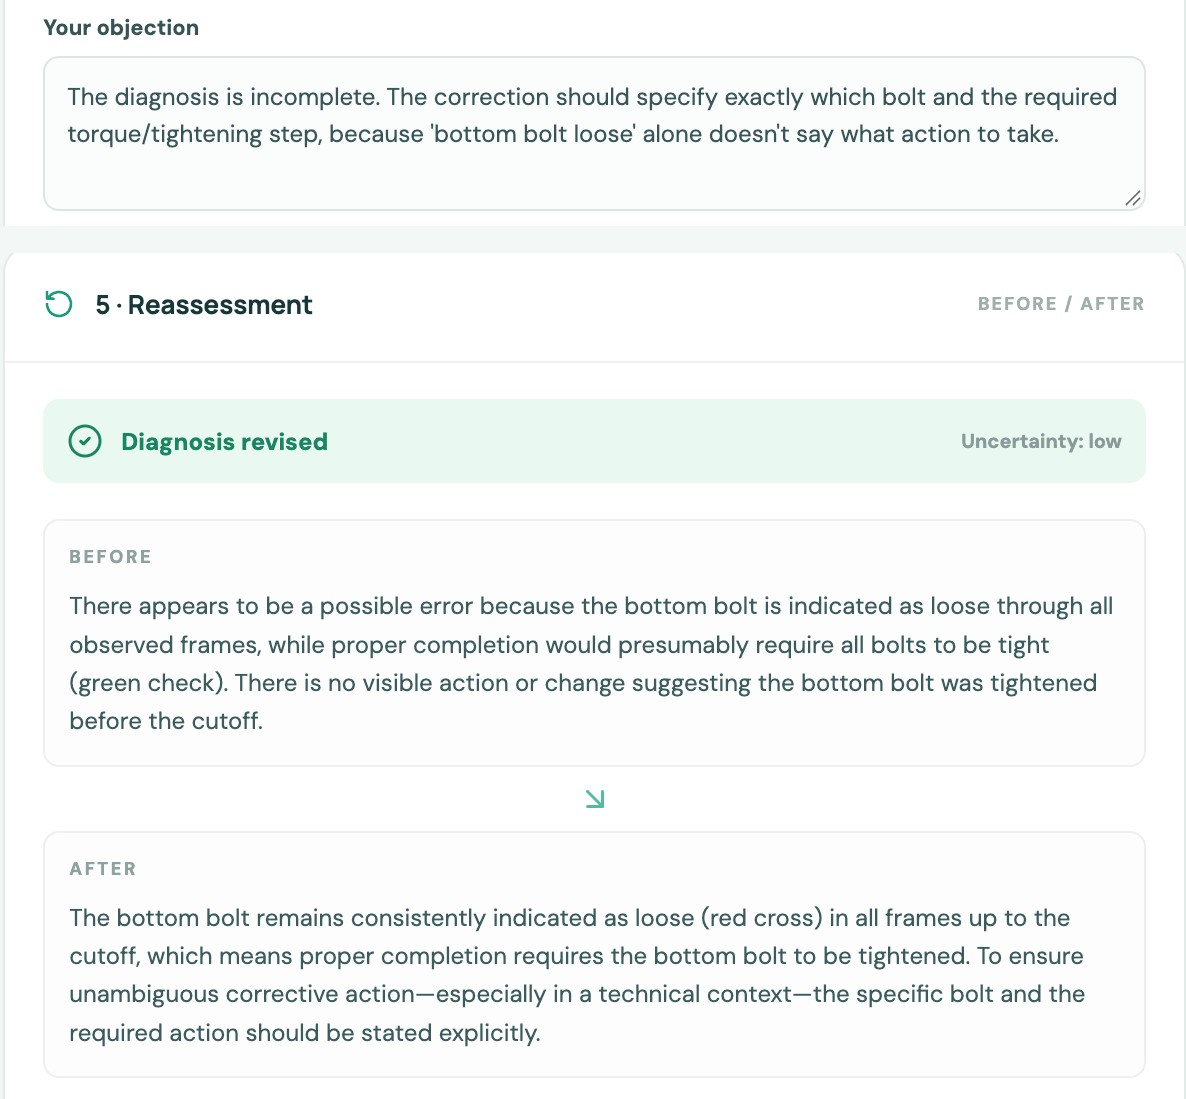
\includegraphics[width=\columnwidth]{figures/ui_reassess.jpg}
\caption{A challenge on the bolts clip. The user objects that the correction is too vague to act on; the model revises while keeping its reading of the frames (the bottom bolt is still the loose one).}
\Description{A screenshot of the challenge and reassessment panels. The objection reads: the diagnosis is incomplete and the correction should specify exactly which bolt and the tightening step. Below, a green banner reads Diagnosis revised, uncertainty low, followed by a Before box describing the bottom bolt as loose and an After box stating that the bottom bolt must be tightened and that the bolt and action should be stated explicitly.}
\label{fig:reassess}
\end{figure}

The contrast with a second objection on the same clip is useful. When I argued only that the correction was too vague to act on, the model revised without changing its reading of the frames: it kept the bottom bolt as the problem and rewrote the suggested check to name the bolt and the tightening step (Figure~\ref{fig:reassess}). So the same clip produced one faithful revision and one unfaithful one, and the difference was whether the objection asked the model to see something that was not there.

\textbf{A supported challenge recovered a missed error.} On the DSLR segment the first diagnosis said the lens was reattached correctly, which contradicts the HoloAssist label. After an objection pointing at the unmatched alignment marks near 17\,s, the model revised, cited frames from that moment, and proposed matching the marks before twisting. I should be clear that I wrote this objection knowing the label. It shows the loop can take in correct feedback; it does not show that users would supply it.

\textbf{Abstention mostly happened at the diagnosis stage.} The occluded clip and a three-second HoloAssist window both returned \emph{insufficient evidence}. When I raised an unresolvable doubt about a clear clip, the model upheld instead of abstaining. That may be the right call, but it means abstain as a challenge outcome was rare.

\textbf{Results were not stable.} The same clip and objection produced different outcomes across runs, and on the graphics-card segment the first diagnosis itself flipped between \emph{possible error} and \emph{no error observed}. For a tool meant to support trust, this matters as much as accuracy.

\textbf{Smaller observations.} The model often cited all 16 frames for one claim, which makes the evidence chips much less useful for checking. Transcript quality also mattered: an early synthetic clip was built so that its audio was cut off mid-sentence, dropping the word ``target,'' and the analysis lost that context; Whisper also misheard ``First I align'' as ``First one align.''

\section{Discussion and Future Work}

\textbf{Evidence needs a support check, not only an ID check.} The bolts case shows that a valid citation can carry a false description. A next step is a separate check that asks whether a cited frame supports the specific sentence, scored by people on a 0/1/2 rubric during evaluation, and possibly by a second model at runtime. Limiting each claim to its two or three most relevant frames would also make the chips worth clicking.

\textbf{Revision should cost evidence.} Right now the model can revise with no new support. One option is to allow \emph{revise} only when the answer cites the user's frame or a frame not cited before, and to have it state what in that frame changed its mind. Re-running the challenge and flagging disagreement between runs would also expose the instability above to the user instead of hiding it.

\textbf{Better use of time.} Sixteen evenly spaced frames can miss a short action. Sampling more densely around the user's selected time, or using models that take video and audio directly, should help. The longer-term setting is live use on smart glasses, where the shared first-person view studied by Teng et al.~\cite{teng2026seeing} could let the user point at the moment they doubt while still holding the part.

\textbf{What I would test first.} The design assumes that people open the evidence. If they do not, RQ1 fails regardless of model quality, and my observation that the model cites every frame suggests they might not. So the first study I would run is a within-subjects comparison of plain advice against advice with evidence links, on HoloAssist segments whose errors are labeled, with some diagnoses deliberately unsupported. I would measure whether participants catch the unsupported ones, how often they click evidence, and how long they take. The second would test RQ2 with misleading objections across repeated runs, to estimate how often the model gives in.

\section{Limitations}

I tested my own system, on six clips, three of which I designed. I wrote objections knowing the reference answers. There were no participants, so nothing here speaks to trust, comprehension, or verification accuracy. Only one model family was used, under rate limits that constrained the number of runs, and the synthetic and HoloAssist results come from different model versions (GPT-4.1 and GPT-4.1-mini), so they are not directly comparable. The HoloAssist audio I used is pitch-shifted, and the segments were chosen because they had a labeled error, which is not representative of real use.

\section{Conclusion}

EvidenceLens makes an AI diagnosis of a physical-task video something a person can open and dispute claim by claim. In my walkthrough the model usually resisted wrong objections, recovered a missed error when given good evidence, and declined to diagnose when the view was blocked. It also once gave in and described frames that did not exist. Making AI advice contestable seems to need two things at once: interfaces that send people to the evidence, and checks that hold the model to what the evidence shows.

\begin{acks}
Use of AI tools: parts of the prototype code and an initial draft of this report were produced with an AI coding assistant. Some walkthrough runs were sent to the prototype's backend through test scripts written by the assistant; the rest were done by hand in the interface. I reviewed, ran, and tested the system, and revised the text. HoloAssist data is used under its CDLA-Permissive-2.0 license and is not redistributed.
\end{acks}

\bibliographystyle{ACM-Reference-Format}
\bibliography{references}

\end{document}
